\documentclass[aps,pra,reprint,amsmath,amssymb,longbibliography,floatfix]{revtex4-2}
\usepackage[utf8]{inputenc}
\usepackage[T1]{fontenc}
\usepackage{booktabs}
\usepackage{array}
\usepackage{graphicx}
\graphicspath{{outputs/paper_v2/figures/}}
\usepackage{xcolor}
\usepackage{hyperref}
\hypersetup{colorlinks=true,linkcolor=blue!60!black,citecolor=blue!60!black,urlcolor=blue!60!black}

\newcommand{\Fi}{F_i}
\newcommand{\nop}{\hat{n}}
\newcommand{\adag}{\hat{a}^\dagger}
\newcommand{\aop}{\hat{a}}
\newcommand{\rhob}{\hat{\rho}_{\mathrm{burn}}}
\newcommand{\DS}{D_S}
\newcommand{\Cb}{C_S^{\mathrm{burn}}}
\newcommand{\nexp}{\langle\nop_i\rangle}

\begin{document}

\title{Intervention-relative control selectors in an open Bose--Hubbard chain:\\
variance, occupation, and the transport boundary}

\author{Kunal Bhatia}
\email{kunal29bhatia@gmail.com}
\affiliation{Independent Researcher, Heidelberg, Germany}
\altaffiliation{ORCID: \href{https://orcid.org/0009-0007-4447-6325}{0009-0007-4447-6325}}
\date{\today}

\begin{abstract}
We ask whether a local observable can serve as a \emph{targeted control handle} in an open
quantum system, and whether the answer depends on the class of intervention applied. Using exact
Lindblad evolution of a one-dimensional open Bose--Hubbard chain ($L\le8$), we show that the local
occupation variance $\Fi=\langle\nop_i^2\rangle-\nexp^2$ identifies the sites whose targeted
perturbation produces the largest finite-horizon response---but only for \emph{number-conserving}
transport interventions. The handle is active precisely when the selected sites enter a
\emph{directed self-draining} regime, which by particle-number continuity is the time-integrated
net outward current; the burn-in current divergence of the selected set predicts the response
($\rho\approx0.9$ at $L=6,7,8$), and the coupling-driven crossover is a current reversal. The
previously proposed redistribution-susceptibility explanation is shown to be non-discriminating
(correlation $\approx0$ with success) and is retired. Under deterministic tilt and random disorder
$\Fi$ outperforms geometry; it generalizes to coherent local detuning (a sign-controlled handle)
but \emph{not} to particle loss, where local occupation $\nexp$ is the operative selector; and
direct bond (hopping) control does not reveal a deeper bond-level handle. The result is a clean,
falsifiable map: $\Fi$ is the selector for $N$-conserving transport-control handles and $\nexp$
for the $N$-changing loss handle, with the boundary set by particle-number conservation.
\end{abstract}

\maketitle

\section{Introduction}
The interplay of tunnelling and on-site interaction in the Bose--Hubbard model underlies much of
cold-atom many-body physics~\cite{fisher1989,jaksch1998,greiner2002,kuhner2000}, and coupling such
systems to an environment---most simply through local dephasing in the
Lindblad framework~\cite{lindblad1976,gorini1976,breuer2002,pichler2010,poletti2012}---drives them
into spatially heterogeneous, far-from-equilibrium states. The deliberate use of dissipation as a
control and state-preparation resource is by now a broad
program~\cite{diehl2008,verstraete2009,sieberer2016,daley2014}. A natural and underexplored
question in this setting is \emph{operational}: can a local structural observable act as a
control handle---does perturbing the sites it selects produce a measurably different future than
perturbing the same budget elsewhere---and is such ``control relevance'' a fixed property of the
observable or a property of the observable \emph{together with} the intervention?

This paper answers both questions for one concrete observable, the local occupation variance
$\Fi$. An earlier version of this study established only that targeting high-$\Fi$ sites with extra
dephasing beats matched-budget random targeting in a ``positive pocket'' of couplings. Here we
(i) identify the dynamical mechanism, (ii) show it is not the redistribution susceptibility
previously invoked, (iii) separate it from geometry under symmetry breaking, and (iv) map how the
operative selector changes as the intervention class is varied---dephasing, coherent detuning,
particle loss, and direct bond control. The central finding is that description privilege is
\emph{intervention-relative}: $\Fi$ is the right selector for number-conserving transport handles,
while local occupation takes over for number-changing loss. All results are exact (no Trotter,
unravelling, or mean-field); the scope is correspondingly limited to small chains, $L\le8$.

\section{Model and methods}
The Hamiltonian for $L$ sites with open boundaries is
\begin{equation}
\hat H=-J\sum_{i}(\adag_i\aop_{i+1}+\mathrm{h.c.})+\frac{U}{2}\sum_i\nop_i(\nop_i-1)
\;\Big(+\sum_i\mu_i\nop_i\Big),
\end{equation}
at half filling $N=\lfloor L/2\rfloor$, local cutoff $n_{\max}=3$; the optional $\mu_i$ implements
tilt/disorder. The density matrix obeys
$\dot{\hat\rho}=-i[\hat H,\hat\rho]+\sum_i\gamma_i(\hat L_i\hat\rho\hat L_i^\dagger-\tfrac12\{\hat L_i^\dagger\hat L_i,\hat\rho\})$,
evolved exactly via the action of the matrix exponential~\cite{scipy2020}. Baseline dephasing
$\hat L_i=\nop_i$ at $\gamma=0.1$; the ground state is evolved for a burn-in $t_{\mathrm{burn}}=5$
to give $\rhob$, on which the selector $\Fi=\langle\nop_i^2\rangle-\nexp^2$ is evaluated and the
top-$k$ sites ($k=\lceil L/3\rceil$) are selected.

\emph{Interventions} (applied after burn-in) define four classes: extra dephasing
($\hat L_i=\nop_i$, $N$-conserving, incoherent), coherent detuning
($\hat H\to\hat H+\mu_{\mathrm{extra}}\sum_{i\in S}\nop_i$, $N$-conserving, coherent), local loss
($\hat L_i=\aop_i$, $N$-changing), and bond modulation ($J_b\to J_b(1+\delta)$, $N$-conserving,
coherent). Loss requires the multi-$N$ space $N\in\{0,\dots,N_0\}$, which is exact (no truncation;
$D=84$ for $L=6$) and reproduces the fixed-$N$ evolution to machine precision at
$\gamma_{\mathrm{loss}}=0$.

\emph{Target and sign convention.} For a selected set $S$ the directed self-drain is
$\DS(\tau)=-\sum_{i\in S}\Delta\nexp(\tau)$, so $\DS>0$ means the selected sites lose occupation.
The Hermitian bond current is
$\hat I_{i,i+1}=-iJ(\adag_i\aop_{i+1}-\mathrm{h.c.})=2J\,\mathrm{Im}\langle\adag_i\aop_{i+1}\rangle$;
because the dephasing dissipator conserves each $\nexp$ exactly, continuity holds,
$d\nexp/dt=\langle\hat I_{i-1,i}\rangle-\langle\hat I_{i,i+1}\rangle$ (verified numerically to
$<10^{-4}$), so $\DS$ \emph{is} the time-integrated net outward current of $S$. The burn-in current
divergence of $S$ is $\Cb=\sum_{i\in S}(\langle\hat I_{i,i+1}\rangle-\langle\hat I_{i-1,i}\rangle)$,
evaluated on $\rhob$. The handle is quantified by the percentile of the selected subset among all
$\binom{L}{k}$ size-$k$ subsets, ranked by clipped local loss (or, for loss, by total system loss
$\Delta N_{\mathrm{tot}}=N_0-\langle\hat N\rangle$). Symmetry between $\Fi$ and geometry is broken by
a deterministic linear tilt and by on-site disorder $\mu_i\sim\mathrm{Uniform}(-\mu_{\max},\mu_{\max})$.

\section{Results}

\subsection{The handle and its regimes}
Targeting the highest-$\Fi$ sites becomes effective above a coupling-dependent onset: at $\tau=3$
the top-$\Fi$ subset rises from below the median at $J/U=0.12$ to the top of the all-subset
distribution by $J/U\simeq0.24$--$0.30$ for $L=6,7,8$ [Fig.~\ref{fig:mech}(a)]. The exhaustive
percentiles reproduce those reported previously (e.g.\ $L=8$, $J/U=0.20$ gives $34/68/71$ at
$\tau=1,2,3$), establishing that the same effect is under study. The remainder of the paper asks
what variable controls this onset.

\begin{figure*}[tbp]
\centering
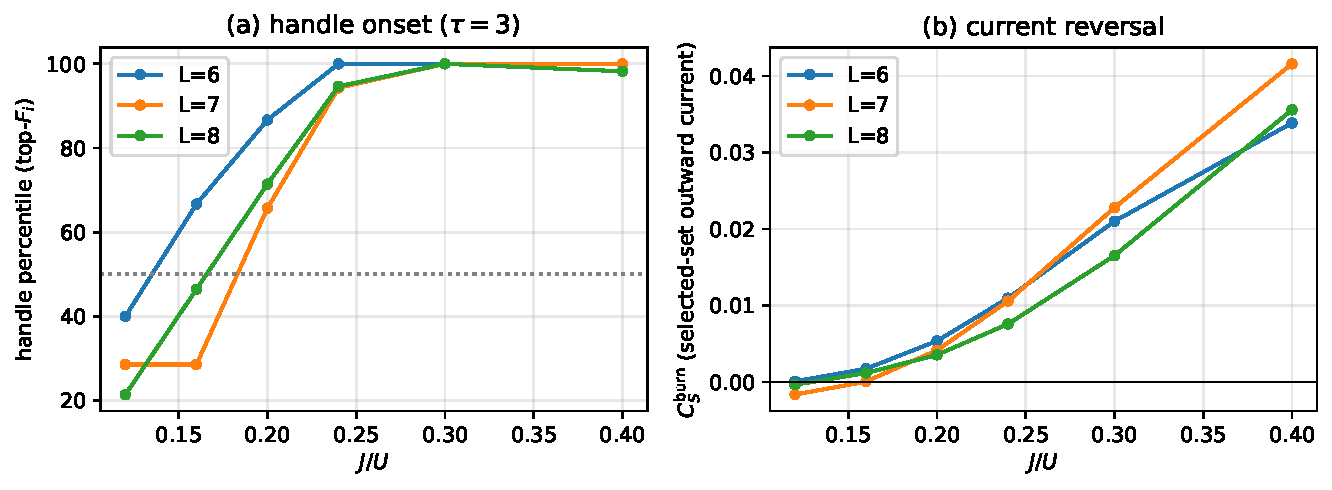
\includegraphics[width=0.92\linewidth]{figA_mechanism.pdf}
\caption{\textbf{Directed self-drain and the current-reversal crossover.}
(a) Handle percentile of the top-$\Fi$ subset vs $J/U$ ($\tau=3$, $L=6,7,8$).
(b) Burn-in outward current $\Cb$ of the selected set vs $J/U$: it crosses zero
(inward $\to$ outward) near the handle onset---the crossover is a current reversal.}
\label{fig:mech}
\end{figure*}

\subsection{Mechanism: directed self-drain is outward current}
By continuity $\DS$ equals the integrated net outward current of $S$, and the static burn-in
current divergence $\Cb$ predicts both $\DS$ and the handle. Table~\ref{tab:T1} shows
$\rho(\Cb,\DS)\approx0.9$ and $\rho(\Cb,\mathrm{handle})\approx0.94$ at all three sizes;
Fig.~\ref{fig:mech}(b) shows $\Cb$ reversing sign (inward/fill $\to$ outward/drain) at the onset,
and Fig.~\ref{fig:pred} the $\Cb$--$\DS$ correlation. The mechanism is therefore transport, not a
static local property: high-$\Fi$ sites become useful once they sit on an outward-current channel,
and that channel turns on with coupling.

\begin{table}[tbp]
\centering
\caption{Current predictor of the handle, clean chain. $\rho$ is Spearman over all
$(J/U,\tau)$ conditions.}
\label{tab:T1}
\begin{tabular}{lcccc}
\toprule
$L$ & onset $J/U$ ($\tau{=}3$) & $\rho(C_S^{\rm burn},D_S)$ & $\rho(C_S^{\rm burn},\text{handle})$ & max $|$cont.\ err$|$ \\
\midrule
6 & 0.24 & $+0.91$ & $+0.94$ & $<10^{-4}$ \\
7 & 0.30 & $+0.91$ & $+0.95$ & $<10^{-4}$ \\
8 & 0.30 & $+0.89$ & $+0.92$ & $<10^{-4}$ \\
\bottomrule
\end{tabular}

\end{table}

\begin{figure}[tbp]
\centering
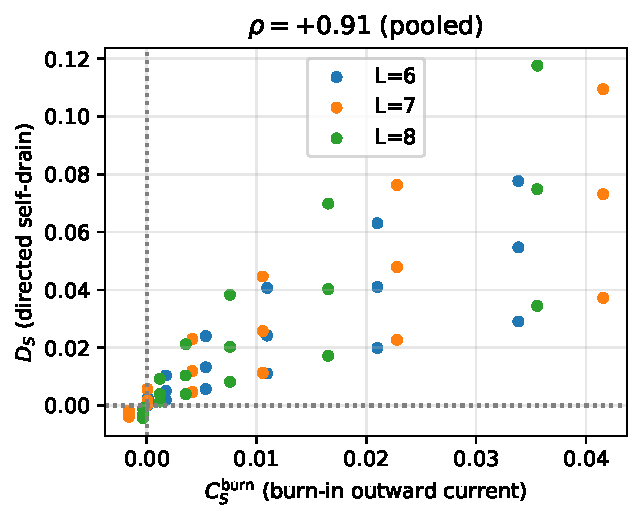
\includegraphics[width=0.82\linewidth]{figB_predictor.pdf}
\caption{Directed self-drain $\DS$ versus burn-in outward current $\Cb$ (pooled $L=6,7,8$);
the two track each other, and both change sign together.}
\label{fig:pred}
\end{figure}

\subsection{The previous explanation, retired}
The earlier account attributed the handle to $\Fi$ tracking a redistribution susceptibility. That
correlation is real but \emph{non-discriminating}: it is comparably large in every regime,
including where the handle fails, so its correlation with actual success is $\approx0$
(Table~\ref{tab:T2}). We therefore retire it as the mechanism (retaining it only as a
necessary-but-not-sufficient fact). A naive ``transport freezes at low $J/U$'' picture is likewise
not supported: the static bond coherence varies only weakly across the studied range, so the
operative change is the \emph{direction} of the response, captured by $\Cb$, not the presence of
transport.

\begin{table}[tbp]
\centering
\caption{The redistribution-susceptibility correlation does not predict handle success
($\rho\approx0$), though its per-condition value stays high in both low-coupling and pocket
regimes.}
\label{tab:T2}
\begin{tabular}{lccc}
\toprule
$L$ & $\rho(\text{handle},\,F_i\!\leftrightarrow\!\chi^{\rm redist})$ & $\langle\text{corr}\rangle$ low-$J/U$ & $\langle\text{corr}\rangle$ pocket \\
\midrule
6 & $-0.03$ & $0.85$ & $0.81$ \\
7 & $+0.09$ & $0.65$ & $0.80$ \\
8 & $-0.26$ & $0.71$ & $0.76$ \\
disorder & $+0.02$ & -- & -- \\
\bottomrule
\end{tabular}

\end{table}

\subsection{Beyond geometry: dephasing under symmetry breaking}
In the clean reflection-symmetric chain $\Fi$ coincides with geometric centrality, so the two must
be separated by breaking the symmetry. Under both deterministic tilt and random disorder the
top-$\Fi$ selector beats a geometric selector (Table~\ref{tab:T3}, Fig.~\ref{fig:geo}); the
separation is sharpest where $\Fi$ and geometry pick the most different sites (disorder,
within-shell overlap $<0.5$: $95.6$ vs $37.3$). Directed self-drain predicts the handle within the
disorder ensemble ($\rho\simeq0.65$ over all rows). The crossover location is not universal:
strong tilt or disorder supplies directed current at all couplings, so the control parameter is the
directed current itself, not $J/U$.

\begin{figure}[tbp]
\centering
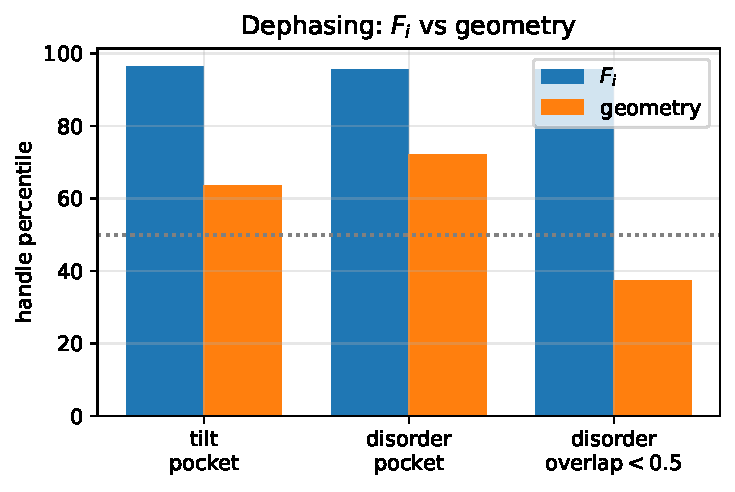
\includegraphics[width=0.86\linewidth]{figC_geometry_dephasing.pdf}
\caption{Dephasing handle percentile, $\Fi$ vs geometry, in the pocket and (disorder) where the
two selectors most disagree. $\Fi$ wins; geometry collapses below the median at low overlap.}
\label{fig:geo}
\end{figure}

\begin{table}[tbp]
\centering
\caption{Geometry separation for both $N$-conserving channels. ``low-overlap'' restricts to
disorder realizations with $\Fi$--geometry overlap $<0.5$ in the pocket.}
\label{tab:T3}
\begin{tabular}{llccc}
\toprule
channel & breaking & overlap & handle pct $F_i$ vs geo (pocket) & low-overlap $F_i$ vs geo \\
\midrule
dephasing & tilt & 0.29 & 96.5 vs 63.7 & -- \\
dephasing & disorder & 0.52 & 95.4 vs 72.1 & 95.6 vs 37.3 \\
detuning & tilt & -- & 68.5 vs 44.6 & -- \\
detuning & disorder & -- & 70.9 vs 58.8 & 49.8 vs 34.6 \\
\bottomrule
\end{tabular}

\end{table}

\subsection{Generality: coherent detuning}
Replacing the dissipative dephasing handle with a coherent local detuning
$\hat H\to\hat H+\mu_{\mathrm{extra}}\sum_{i\in S}\nop_i$ yields a sign-controlled handle
[$+\mu$ drains, $-\mu$ fills; Fig.~\ref{fig:det}(a)] that again beats geometry under symmetry
breaking (Table~\ref{tab:T3}). Thus $\Fi$ is a \emph{general} $N$-conserving transport-control
selector, not a dephasing-specific one. The mechanistic predictor, however, bifurcates: for
dephasing $\Cb$ \emph{reads} the pre-existing current ($\rho\approx0.7$--$0.9$), whereas detuning
\emph{imposes} its own current and $\Cb$ is correspondingly weaker
($\rho\simeq0.46$ tilt, $0.55$ disorder).

\begin{figure*}[tbp]
\centering
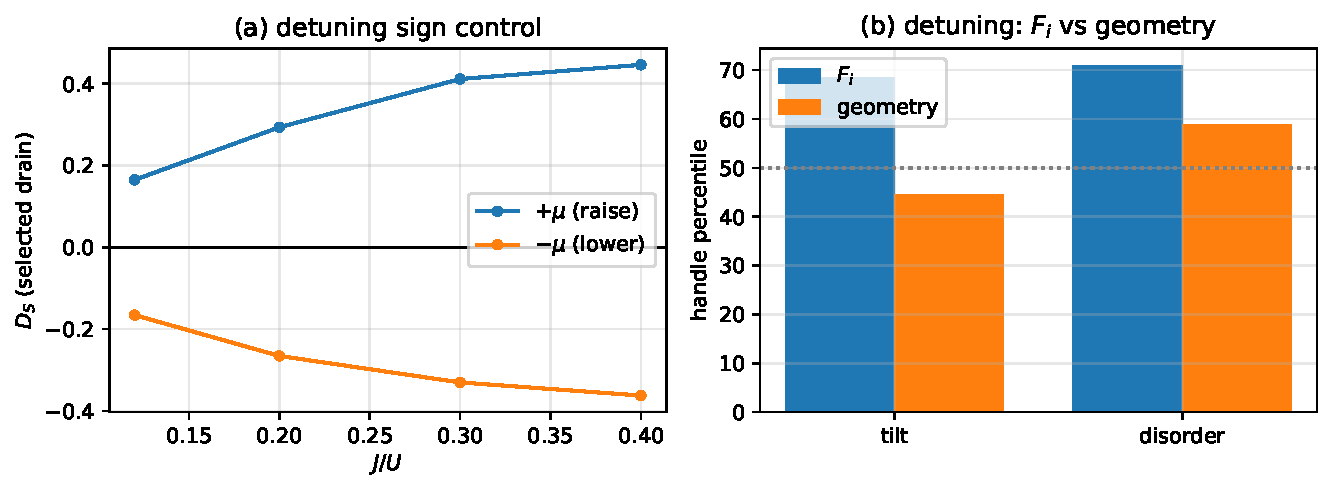
\includegraphics[width=0.92\linewidth]{figD_detuning.pdf}
\caption{\textbf{Coherent detuning.} (a) Selected-site drain $\DS$ vs $J/U$ for $\pm\mu$: raising
the on-site energy drains, lowering fills---a sign knob absent for dephasing.
(b) Detuning handle percentile, $\Fi$ vs geometry, under tilt and disorder: $\Fi$ wins.}
\label{fig:det}
\end{figure*}

\subsection{The boundary: particle loss}
Local amplitude damping ($\hat L_i=\aop_i$) changes $N$; the natural target is the total system
loss $\Delta N_{\mathrm{tot}}$. Here $\Fi$ is \emph{not} operative: local occupation is the best
predictor (Table~\ref{tab:T4}, Fig.~\ref{fig:loss}), decisively so under symmetry breaking, where
$\rho(\Delta N_{\mathrm{tot}},\langle\nop_i\rangle)=+0.998$ versus $+0.73$ for $\Fi$ in the
realizations where the two selectors separate, and the maxn selector reaches the $99.6$th
percentile versus $84.9$ for $\Fi$. Physically, loss directly removes particles from occupied
sites, so the operative variable is occupation; $\Fi$'s residual loss-predictive power is only its
clean-chain correlation with $\langle\nop_i\rangle$. The boundary between the two selectors is thus
\emph{transport-modulation vs.\ particle-removal}---equivalently, particle-number conservation.

\begin{table}[tbp]
\centering
\caption{Loss is occupation-driven. Spearman of $\Delta N_{\mathrm{tot}}$ with each candidate
selector; ``separated'' restricts to realizations where $\Fi\ne\mathrm{maxn}$.}
\label{tab:T4}
\begin{tabular}{lcccc}
\toprule
predictor of $\Delta N_{\rm tot}$ & $\langle n_i\rangle$ & $F_i$ & current & geometry \\
\midrule
clean $L=6$ & $+0.95$ & $+0.87$ & $+0.87$ & $+0.86$ \\
sym-broken (separated) & $+0.998$ & $+0.73$ & -- & $+0.19$ \\
\bottomrule
\end{tabular}

\end{table}

\begin{figure}[tbp]
\centering
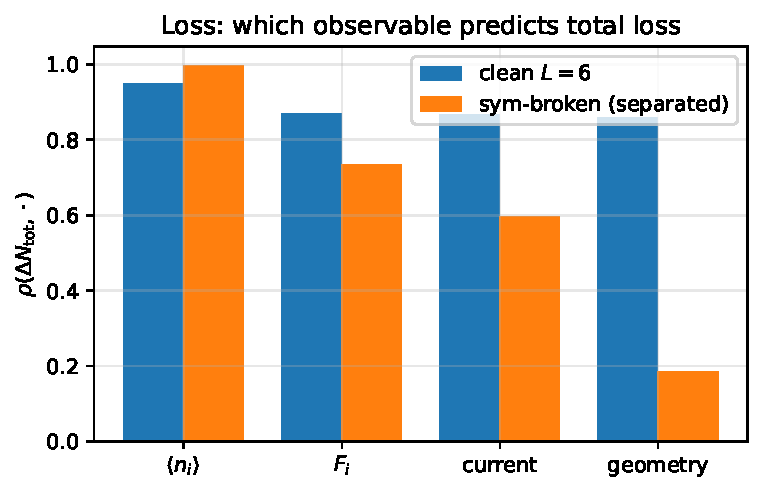
\includegraphics[width=0.78\linewidth]{figE_loss.pdf}
\caption{Which observable predicts total particle loss. Occupation dominates; under symmetry
breaking it is near-perfect while geometry is irrelevant.}
\label{fig:loss}
\end{figure}

\subsection{Site versus bond control}
Since current is a bond quantity, we tested whether the handle is fundamentally bond-level by
modulating the hopping on selected bonds. Using the baseline-clean (induced) per-endpoint drain as
the target, no bond observable predicts the effect (best $|\rho|=0.19$); on the
baseline-confounded total, the site-derived endpoint-$\Fi$ is not beaten by bond coherence or bond
current (Table~\ref{tab:T5}). The site-level description is therefore kept: bond control does not
expose a deeper bond-level handle, and the strong $\Fi$--bond-coherence correlation is a
correlation, not a better selector.

\begin{table}[tbp]
\centering
\caption{Bond/hopping modulation. ``induced'' is the per-endpoint drain change due to the
modulation (the clean bond-control signal); ``total'' is baseline-confounded.}
\label{tab:T5}
\begin{tabular}{lcc}
\toprule
bond selector & $\rho$ (induced) & $\rho$ (total) \\
\midrule
endpoint-$F_i$ (site-derived) & $-0.10$ & $+0.87$ \\
bond coherence & $+0.00$ & $+0.60$ \\
$|$bond current$|$ & $+0.07$ & $-0.83$ \\
endpoint occupation & $-0.19$ & $+0.86$ \\
\bottomrule
\end{tabular}

\end{table}

\subsection{Observer-geometry reanalysis (supporting)}
A separate pre-registered reanalysis of the same simulation data, using an observer-geometry
framework, provides supporting structure. Two outcomes are earned and reported: observer subspaces
converge monotonically as the chain thermalizes, and the choice of scoring rule changes which site
is ``optimal'' in every cell---both consistent with the redistribution picture. A third, earlier
``predictive--causal dissociation'' result is \emph{not} retained as a finding: its headline rate
($\sim0.90$) is dominated by a self-correlation artifact (the prediction target lies inside the
observer family), and the honest rate once that observer is excluded is $\sim0.52$. We report it
here only as a limitation.

\section{Discussion}
The results assemble into a single map (Table~\ref{tab:T6}): the operative control selector is not
a fixed property of the chain but depends on the allowed intervention. For number-conserving
handles---incoherent dephasing and coherent detuning---the variance $\Fi$ selects the
transport-active, directed-self-draining sites, and the effect is mechanistically the integrated
outward particle current. For the number-changing loss handle the operative selector is local
occupation. Geometry is, in every case, at most a correlate. This is a concrete, falsifiable
instance of \emph{intervention-relative description privilege}: the same physical system selects
different useful descriptions depending on the class of control applied, with the boundary set by a
clean physical distinction (transport modulation versus particle removal). The picture connects
naturally to dissipation engineering and to Zeno-type throttling of coherent
transport~\cite{diehl2008,daley2014}, while remaining agnostic about which microscopic relaxation
mode carries the current---an explicit open question.

\begin{table}[tbp]
\centering
\caption{The intervention-relative map: operative selector by intervention class.}
\label{tab:T6}
\begin{tabular}{lcc>{\bfseries}c}
\toprule
intervention & conserves $N$? & coherent? & operative selector \\
\midrule
dephasing & yes & no & $F_i$ \\
 detuning & yes & yes & $F_i$ \\
local loss & no & no & $\langle n_i\rangle$ \\
 bond hopping mod. & yes & yes & site-level $F_i$ (not bond) \\
\bottomrule
\end{tabular}

\end{table}

\section{Conclusion}
In exact small open Bose--Hubbard chains, local number variance is the operative control selector
for number-conserving transport interventions (dephasing and detuning), while local occupation is
the operative selector for number-changing loss; geometry is not fundamental; and the handle
operates only in the directed self-draining regime, which is the integrated outward particle
current, with the coupling crossover a current reversal. The natural next steps---a Liouvillian
spectral decomposition to identify which slow mode carries the current, and approximate methods
(quantum trajectories, matrix-product operators) to test persistence at larger $L$---are left for
future work. We make no claim beyond the exact, small-$L$ regime studied here: not the
thermodynamic limit, not a universal control law, and not laboratory realization.

\appendix
\section{Numerical validation}
Time evolution is exact via Krylov/Pad\'e matrix-exponential action; the sparse and dense code
paths agree to $\sim10^{-15}$. For loss, the multi-$N$ construction is exact (it includes all
sectors $N\le N_0$ reachable under loss), reproduces the fixed-$N$ occupations to $2\times10^{-16}$
at $\gamma_{\mathrm{loss}}=0$, preserves trace and positivity, and gives a particle number that
decreases monotonically and linearly in $\gamma_{\mathrm{loss}}$. Continuity
$d\nexp/dt=\langle\hat I_{i-1,i}\rangle-\langle\hat I_{i,i+1}\rangle$ is verified to $<10^{-4}$
(finite difference), and the per-bond-$J$ Hamiltonian reduces to the scalar-$J$ Hamiltonian when
all $J_b$ are equal. All headline numbers are computed directly from the deposited simulation
outputs; code and data are available with the manuscript.

\bibliography{refs}
\end{document}
